\documentclass{article}
\usepackage[utf8]{inputenc}
\usepackage[english]{babel}
\usepackage{geometry}
\usepackage{amssymb}
\usepackage{amsfonts}
\usepackage{dsfont}
\usepackage{float}
\usepackage{graphicx}
\usepackage{wrapfig}
\usepackage{mathtools}
\usepackage{bbm}
\usepackage{amsthm}
\usepackage{ifthen}
\usepackage{graphicx}
\usepackage{hyperref}
\usepackage{tcolorbox}
\usepackage[ruled,vlined]{algorithm2e}
\usepackage{tikz}

\usepackage{caption}
\usepackage{subcaption}

%%%%%%%% box %%%%%%%%
\definecolor{mycolor}{rgb}{0.122, 0.435, 0.698}% Rule colour
\makeatletter
\newcommand{\mybox}[1]{%
	\setbox0=\hbox{#1}%
	\setlength{\@tempdima}{\dimexpr\wd0+13pt}%
	\begin{tcolorbox}[colframe=blue,boxrule=0.5pt,arc=4pt,
		left=6pt,right=6pt,top=6pt,bottom=6pt,boxsep=0pt,width=\@tempdima]
		#1
	\end{tcolorbox}
}
%%%%%%%%





\DeclarePairedDelimiter{\ceil}{\lceil}{\rceil}

\newcommand{\ca}[1]{\mathcal{#1}}
\newcommand{\bb}[1]{\mathbb{#1}}
\newcommand{\p}{\mathbb{P}}
\newcommand{\evento}[1]{\left\{ \textit{``#1''} \right\}}
\newcommand{\comillas}[1]{``#1''}
\newcommand{\set}[1]{\left\{#1\right\}}
\newcommand{\parent}[1]{\left(#1\right)}
\newcommand{\parentCuad}[1]{\left[#1\right]}
\newcommand{\borel}{\ca{B}(\bb{R}^d)}
\newcommand{\Rd}{\bb{R}^d}
\newcommand{\R}{\bb{R}}
\newcommand{\infNorm}[1]{||#1||_\infty}
\newcommand{\condExp}[2]{\bb{E}(#1|#2)}
\newcommand{\ind}[1]{\mathbbm{1}_{#1}}
\newcommand{\esp}[1]{\bb{E}\barras{#1}}
\newcommand{\indep}{\rotatebox[origin=c]{90}{$\models$}}
\newcommand{\pe}{$(\Omega, \ca{F}, \p)\ $}
\newcommand{\vc}[1]{\langle #1 \rangle}
\newcommand{\gb}[1]{\overline{\widehat{#1}}}
\newcommand{\barras}[1]{\left| #1 \right|}
\newcommand{\integral}{\int_{t_i}^{t_{i+1}}}
\newcommand{\ug}[1]{\widehat{\ca{U}}_{#1}}
\newcommand{\vg}[1]{\widehat{\ca{V}}_{#1}}
\newcommand{\zg}[1]{\widehat{\ca{Z}}_{#1}}
\newcommand{\norm}[1]{\left\lVert#1\right\rVert}
\newcommand{\X}{\ca{X}}
\newcommand{\xscheme}[1]{X_{t_{#1}}^{\pi}}
\newcommand{\prom}[1]{\langle #1 \rangle}


\begin{document}
%%%



%%% Portada %%%
\begin{titlepage}
	\centering
	{\bfseries\LARGE Universidad De Chile \par}
	\vspace{1cm}
	{\scshape\Large Facultad de Ciencias Físicas y Matemáticas \par}
	\vspace{3cm}
	{\scshape{\Huge \textbf{LDA con datos de Twitter}}\\
		Probabilidades y Estadística en el Análisis de Datos \par}
	\vfill
	{\Large  Javier Castro Medina\par}

	\vfill
	{\Large Julio 2021 \par}
\end{titlepage}
%%% Portada %%%
\newpage
%%%%
\section{Introducción}
En este informe se documenta lo realizado en el proyecto: LDA con datos de twitter. En este se cuenta con un set de datos consistente en tweets en formato texto, se busca aplicar el algoritmo LDA de topic modelling del cual se habla más adelante. En la primera presentación de avance de proyecto, se mostró el formato de los datos y se expuso un pequeño análisis a los primeros set de datos que se recopilaron. En la segunda presentación se expuso el algoritmo LDA y se aplicó, con la ayuda de la librería \texttt{gensim}, sobre los tweets de la cuenta \texttt{@gabrielboric} mostrando resultados preliminares. En este informe se especifica en cierto nivel de detalle el preprocesamiento de los tweets, se explica el algoritmo utilizado junto a la métrica que se usa para evaluar su desempeño y además, se muestra cómo se fue optimizando esta métrica en función de los parámetros del modelo\\

La motivación de este proyecto partió con la idea de identificar discursos de odio en la red social Twitter. Pero, una vez hecho el análisis exploratorio de los datos, surge y se prefiere la idea de aplicar algoritmos de topic modelling puesto que era algo más concreto a realizar sobre el data set. Es así como se comienzan a definir distintos objetivos e ideas a medida se iban revisando y procesando los datos, el objetivo principal es capturar de la mejor manera posible, en base a métricas, los temas que principalmente se discutan en un set de tweets. Como se trabajó con tweets de la cuenta \texttt{@gabrielboric}, se esperaba que por lo menos se pueda identificar un tópico con carácter político. Otra hipótesis es que en general, como Twitter es usado para discutir temas nacionales, los tópicos encontrados en un set de tweets entre $2019-2021$ tengan también tópicos con tintes políticos puesto que en esos años han habido varias discusiones y procesos políticos, además, claramente, deberíamos encontrar algunos relativos a la pandemia.\\

En la sección $2$ se habla del análisis exploratorio que se realizó sobre los primeros data sets y cómo fueron recolectados, en la sección $3$ se discute el algoritmo LDA definiendo además la métrica utilizada en su evaluación, en la sección $4$ mostramos la aplicación del algoritmos a nuestros data sets y, finalmente, en la sección $5$ se concluye y discuten ideas para la expansión del proyecto.

\section{Análisis Exploratorio}
Para la obtención de tweets se usa la librería \texttt{twint}\footnote{\href{https://github.com/twintproject/twint}{github.com/twintproject/twint}}. Esta librería es simple de usar y permite obtener una gran cantidad de datos con la opción de almacenarlos en formato \texttt{csv}. En las Figuras \ref{fig: twint_example1_informe} y \ref{fig: twint_example2_informe} se muestra, a grandes rasgos, el código que se necesita para obtener los datos utilizados en este trabajo.    


\begin{figure}[H]

	\centering
	\subfloat[]{
			\label{fig: twint_example1_informe}
			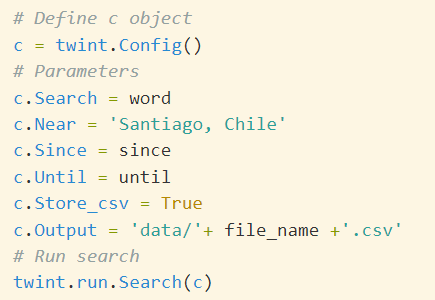
\includegraphics[scale=.4]{../imgs/twint_example1_informe.png}
	}
	%\hfill
	\subfloat[]{
			\label{fig: twint_example2_informe}
			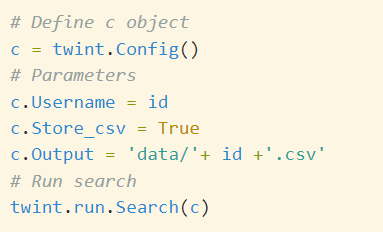
\includegraphics[scale=.4]{../imgs/twint_example2_informe.png}
	}
	\caption{A la izquierda se buscan y guardan tweets creados al rededor de Santiago entre las fechas \texttt{since} y \texttt{until} que además contengan la palabra \texttt{word}. A la derecha se obtienen y guardan los tweets de la cuenta \texttt{id}. En inglés este proceso se denomina \textbf{scrapping tweets}}.
\end{figure}

En la primera parte del proyecto se realiza un proceso de adaptación a la librería \texttt{twint} y el formato de los datos que permite obtener, además, se realiza un análisis superficial a los datos recolectados en la fase inicial del proyecto. Se decide trabajar sólo con tweets en Santiago, esto porque en tal sector hay una población más grande y por lo tanto, una probabilidad más alta de encontrar cuentas de Twitter con respecto a otros lugares. Lo que queda de esta sección se divide en dos partes, en la primera se mostrarán worclouds y en la segunda gráficos de la frecuencia de tweets diarios para distintos set de datos.

\begin{remark}
	Otra razón por la cual fijar el lugar geográfico en la obtención de tweets es disminuir la complejidad del proyecto, puede ser un aspecto a considerar en una tarea de mayor escala en la que se tome en cuenta la variable espacial de nuestros datos.	
\end{remark}

\subsection{Wordclouds}
	Se muestran las wordclouds asociadas a tres set de tweets (o datos) distintos. Por un lado tenemos dos hitos importantes en Chile, el primero es el estallido social del $18$ de octubre del $2019$ y el segundo es el día de la mujer del $2020$. El tercero contiene los tweets que contienen la palabra \comillas{piñera} y fueron creados durante el $2020$.
	
	
	
	
   	\begin{figure}[H]
   		\centering
   		\subfloat[]{
	   		\begin{minipage}{0.33\textwidth}
	   			\centering
	   			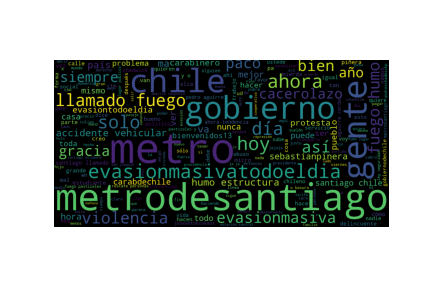
\includegraphics[width=\textwidth]{../imgs/wordcloud_santiago_estallido1.png}
	   		\end{minipage}
   			\label{fig: estallido}
   		}
   		%\hfill
   		\subfloat[]{
	   		\begin{minipage}{0.33\textwidth}
	   			\centering
	   			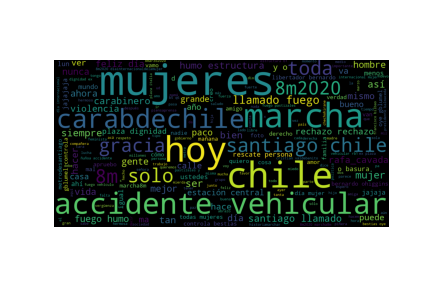
\includegraphics[width=\textwidth]{../imgs/wordcloud_santiago_8M.png}
	   		\end{minipage}
   		\label{fig: mujer}
		}
		%\vfill
		\subfloat[]{
			\begin{minipage}{0.33\textwidth}
				\centering
				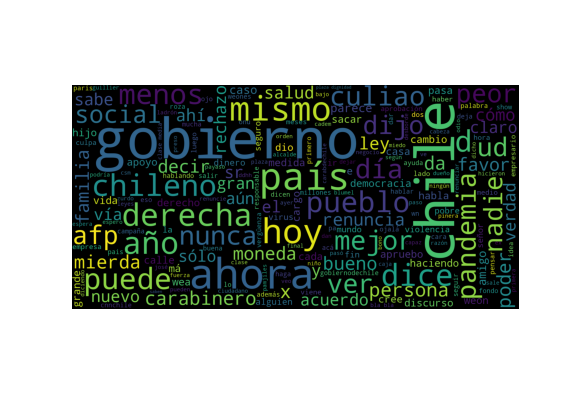
\includegraphics[width=\textwidth]{../imgs/wordcloud_santiago_pinera_2020.png}
			\end{minipage}
		\label{fig: pinera}
		
		}
		\caption{De izquierda a derecha: estallido social, día de la mujer y tweets que contienen la palabra \comillas{piñera}.}
   	\end{figure}
   Para encontrar los tweets del estallido y el día de la mujer sólo se especificaron las fechas y el lugar, el campo \texttt{c.Search} que aparece en la Figura \ref{fig: twint_example1_informe} se deja vacío. En cambio, para los tweets con \comillas{piñera}, se debe usar \texttt{c.Search = 'piñera'}. Las palabras \textbf{metrodesantiago} y \textbf{evasionmasivatodoeldía} que aparecen en \ref{fig: estallido} corresponden a hashtags que estuvieron presentes en Twitter durante los días previos al estallido. En la Figura \ref{fig: mujer} observamos las palabras \textbf{mujeres} y \textbf{marcha}, esto sucede porque en esa fecha ocurre la marcha en conmemoración del día de la mujer que, como vemos, tiene impacto en redes sociales como Twitter. En la Figura \ref{fig: pinera} se destacan las palabras \textbf{gobierno}, \textbf{Chile} y \textbf{derecha} que se relacionan bastante con lo que representa la palabra \comillas{piñera}. En las tres wordclouds se encuentran palabras bastante esperables y que guardan estrecha relación con el contexto social en el cual fueron creados los tweets, esta es una señal que confirma que nuestros datos tienen sentido con su variable temporal.
    
\subsection{Series de tiempo}
Se exponen series de tiempo relativas a la cantidad de tweets diarios que contengan cierta palabra clave. Acá trabajamos con dos set de tweets, por un lado tenemos uno de la sección anterior, asociado a la palabra \comillas{piñera}, y por otro contamos con los tweets que contienen la palabra \comillas{covid} y que fueron creados durante el año $2020$.
\begin{figure}[H]
	\centering
	\subfloat[]{
		\label{fig: serie_covid_2020}
		\begin{minipage}{0.45\textwidth}
			\centering
			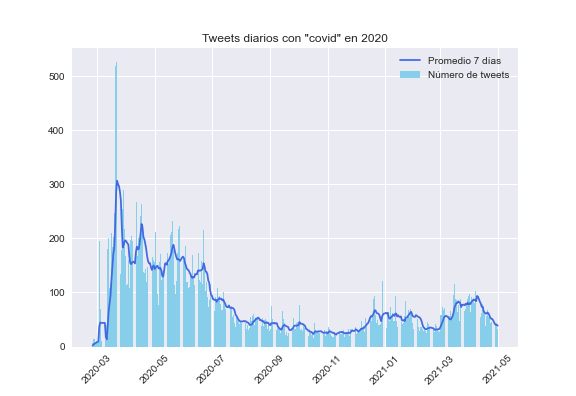
\includegraphics[width=\textwidth]{../imgs/serie_covid_2020.png}
		\end{minipage}
	}
	\subfloat[]{
		\label{fig: serie_pinera_2020}
		\begin{minipage}{0.45\textwidth}
			\centering
			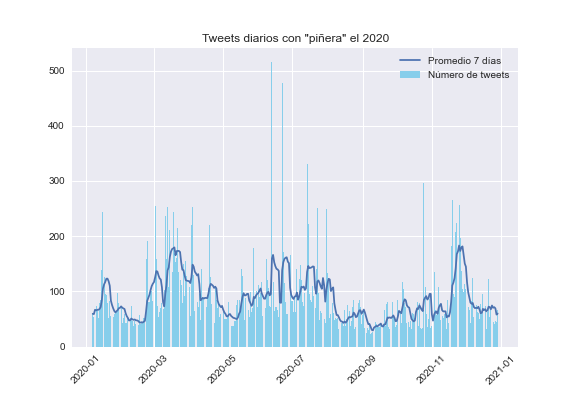
\includegraphics[width=\textwidth]{../imgs/serie_pinera_2020.png}
		\end{minipage}
	}
	\caption{Cantidad de tweets diarios con la palabra \comillas{covid} (a) y \comillas{piñera} (b).}
\end{figure}



En la Figura \ref{fig: serie_covid_2020} vemos que la curva que se genera al suavizar tomando media móvil de siete días es similar a la curva de casos diarios de covid en Chile (también suavizada), pero adelantada en tiempo. El primer peak de los casos diarios ocurrió al rededor de junio \footnote{\href{https://www.google.com/search?client=firefox-b-d&q=covid+chile}{Link a los casos diarios covid en Chile según Google.}}, mientras que en \ref{fig: serie_covid_2020} esto ocurre en marzo cuando todo estaba comenzando. Aproximadamente, en ambas curvas, durante los siguientes seis meses se ve una tendencia a la baja. Esta especie de carácter predictivo de la curva \ref{fig: serie_covid_2020} no es sostenible en el tiempo porque si bien los casos aumentaron hasta superar el primer peak, en Twitter sólo se ve un aumento relativamente pequeño en la cantidad de tweets durante enero. Por otra parte, el peak más alto en \ref{fig: serie_covid_2020} corresponde al día $21$ de marzo del $2020$, en esta fecha se informa la primera muerte por covid en Chile\footnote{\href{https://www.cnnchile.com/coronavirus/hitos-claves-covid-19-chile-mundo-cronologia_20200505/}{Cronología covid-19 en Chile (CNN Chile)}}.\\

Con respecto a la Figura \ref{fig: serie_pinera_2020}, observamos que la cantidad de tweets que hablan de Piñera es relativamente constante en el tiempo, con un promedio de $86$ tweets diarios, y sin una tendencia marcada. 


\section{Latent Dirichlet Allocation aplicado a datos de Twitter}
	Este algoritmo cae en la categoría del \textbf{Topic Modelling} en la cual se busca, a partir de grandes data sets de texto, encontrar tópicos latentes en estos, cosa que sería imposible de hacer \comillas{a mano}. Para este modelo se necesita un set de palabras $V$ y de tópicos $K$, que sin perdida de generalidad denotamos como $K=\set{1,...,K}$. Los tópicos se modelan como distribuciones de probabilidad sobre el conjunto de palabras $V$. Si bien este algoritmo tiene una fase generativa, su objetivo es calibrar parámetros $\alpha\in [0,1]^{K}$ y $\beta\in[0,1]^{K\times V}$ optimizando cierta cantidad. La idea es, dada una \textit{initial guess} o prior de $\alpha$ y $\beta$, generar palabras con el siguiente algoritmo:
	
	\begin{itemize}
		\item Se samplea una distribución sobre tópicos $\theta\sim Dir(\alpha, K)$. Notar que $\sum_{i=1}^K \theta = 1$. $Dir$ es la distribución \href{https://en.wikipedia.org/wiki/Dirichlet_distribution}{Dirichlet}.
		\item Dado $\theta$, se samplea un tópico $t\sim\theta$.
		\item Dado el tópico $t$, se samplea una palabra $w\sim\beta_{t\cdot}$.
	\end{itemize}
	
	\begin{remark}
		Este algoritmo nos permite interpretar los parámetros del modelo. $\theta\in\R^{K}$, que sólo depende de $\alpha$, corresponde a que tan relevante es cada tópico. En cambio, $\beta\in[0,1]^{K\times V}$ modela como se distribuye cada tópico sobre el set de palabras. 
	\end{remark}
	
	Lo anterior permite samplear una $(1)$ palabra, también asumimos que los sampleos son independientes. Consideremos ahora una palabra $w_n$, luego, la probabilidad de generar esta palabra se puede calcular como,
	
	\begin{align*}
		p(w_n|\alpha, \beta) &= \sum_{t\in K} p(w_n|\alpha,\beta,t)p(t|\alpha,\beta)
		= \sum_{t\in K} p(w_n|\beta,t)\int p(t|\alpha,\beta,\theta)p(\theta|\alpha,\beta)d\theta\\
		&= \sum_{t\in K} p(w_n|\beta,t)\int p(t|\theta)p(\theta|\alpha)d\theta.
	\end{align*}
	Donde usamos probabilidades totales y que, según nuestro modelo, $p(w_n|\alpha,\beta,t)=p(w_n|\beta,t)$, $p(t|\alpha,\beta,\theta)=p(t|\theta)$ y $p(\theta|\alpha,\beta)=p(\theta|\alpha)$. Usando la independencia vemos que para $w=(w_1,...,w_N)$,  
	\begin{align*}
		p(w|\alpha,\beta) &= \int p(\theta|\alpha)\parent{\prod_{n=1}^N \sum_{t\in K} p(w_n|t,\beta)p(t|\theta)} d\theta.
	\end{align*}
	
	El calculo anterior tiene razones Bayesianas de ser, esto porque permite calcular la distribución a posteriori de $(\theta, t)$ la cual se busca maximizar. La distribución que se obtiene es intratable numéricamente por lo cual se sigue un approach MCMC o \textbf{variational Bayes}, ver por ejemplo \cite{LDA03, LDA10}. La implementación de este algoritmo en \texttt{Python} esta dada por la librería \texttt{gensim}\footnote{\href{https://radimrehurek.com/gensim/models/ldamodel.html}{Lda con gensim (link)}}, el código se basa en el script \texttt{onlineldavb.py}\footnote{\href{https://github.com/blei-lab/onlineldavb/blob/master/onlineldavb.py}{Link al repositorio.}} de los autores de \cite{LDA10}. En el citado trabajo, los hiperparámetros cambian un poco asumiendo que la distribución $\beta_{t\cdot}$ de cada tópico $t\in K$ sobre las palabras $V$, es tal que $\beta_{t\cdot}\sim Dir(\eta, |V|)$. Así, los hiperparámetros (o priors) pasan a ser $(\alpha,\eta)$ y de esta forma son tratados por \texttt{gensim}.\\ 
	
	La métrica que se utiliza para medir este tipo de modelos se denomina coherencia, esta se aplica sobre un tópico en particular y se define como el nivel de relación que existe entre las palabras más probables dentro del tópico. En \cite{coherence} y \cite{coherence2} se discute este tema en profundidad. Existen varias formas de modelar esta definición, acá usaremos \texttt{u\_mass} que se escribe como sigue.
	\begin{align*}
		\texttt{u\_mass}(t) := \frac{2}{N(N-1)} \sum_{i=2}^N\sum_{j=1}^{i-1}\log \parent{p(w_i|w_j)}.
	\end{align*}
	Donde $t = (w_1,...,w_N)$ es un tópico que se representa por sus $N$ palabras más probables ordenadas y $p(w_i|w_j)$ se estima con las frecuencias de aparición en el corpus usado para aprender los tópicos. En la práctica lo que se hace es definir $D(w)$ como la frecuencia de aparición de $w$ en el corpus, $D(w,v)$ como la frecuencia de aparición de $w$ junto a al menos una aparición de $v$ y aproximar la cantidad anterior como
	\begin{align}
		\label{eq: umass}
		\texttt{u\_mass}(t) = \frac{2}{N(N-1)} \sum_{i=2}^N\sum_{j=1}^{i-1}\log \parent{\frac{D(w_i,w_j)+\epsilon}{D(w_j)}}.
	\end{align}
	Lo que se está calculando es algo así como un promedio de la probabilidades de $w_i$ condicionada en todas $w_j$ anteriores. Intuitivamente nos dice que tan relacionadas entre si están las palabras dentro del tópico, modelando la relación como probabilidad condicional. El $\epsilon>0$ que aparece en (\ref{eq: umass}) es un artilugio técnico para evitar $\log (0)$ y notar que \texttt{u\_mass} es negativa y mejor cuando es más cercana a $0$.
\section{Datos y Desarrollo del Modelo}
	Se decide trabajar con tweets de una cuenta en específico, esto porque el rango de temas o tópicos tocados por una cuenta es menor o más controlado que al trabajar con tweets de muchas cuentas a la vez. La cuenta que se escoge para partir es \texttt{@gabrielboric}, obtenemos sus tweets hasta junio del $2021$. Las características de este data set se pueden apreciar en las Figuras \ref{fig: boric_tweet_año} y \ref{fig: tabla_boric}.

	
	
	
 	\begin{figure}[H]
 		\centering
 		\subfloat[]{
 			\begin{minipage}{0.44\textwidth}
 				\label{fig: boric_tweet_año}
 				\centering
 				\includegraphics[width=\textwidth]{../imgs/boric_tweet_año.png}
 				%\caption{Tweets por año.}
 			\end{minipage}
 		}
 		\subfloat[]{
 			\begin{minipage}{0.44\textwidth}
 				\centering
 				\label{fig: tabla_boric}
 				\begin{tabular}{ c|c } 
 					\hline
 					\textbf{Total de tweets} & $39405$ \\ 
 					\hline
 					\hline
 					\textbf{Mínimo} & $0$ \\
 					\hline 
 					\textbf{Máximo} & $131$ \\
 					\hline
 					\textbf{Promedio} & $9.14$ \\
 					\hline
 				\end{tabular}
 			\end{minipage}
 		}

 		\caption{Tweets por año (a) y el total de tweets junto a estadísticas de la cantidad diaria de tweets (b).}
 	\end{figure}
	
\subsection{Limpieza y preprocesamiento de datos}
	Los datos que se tienen disponible corresponden a tweets en formato de texto. El procesamiento de base o inicial que se realiza sobre este corpus corresponde a eliminar \textbf{stop words}, links, palabras de largo menor o igual a $3$, caracteres indeseables\footnote{Se eliminaron: \#, comas, signos de exclamación y pregunta, paréntesis y el signo igual.} y finalmente, pasar todas las palabras a minúscula. El procesamiento anterior se realizará siempre y al inicio de todo código, luego de este proceso a nivel de vocabulario, se decide eliminar aquellos tweets con una cantidad de palabras menor a $5$ lo que nos deja con $24218$ tweets. Lo siguiente que se puede hacer es quitar palabras de baja frecuencia, sin quitar estas palabras el diccionario\footnote{Entendemos por diccionario al conjunto de todas las palabras utilizadas en el corpus} resultante tiene un tamaño de $35892$ palabras. En el gráfico a continuación muestra la cantidad de palabras resultantes al variar este parámetro.
	
	\begin{figure}[H]
		\centering
		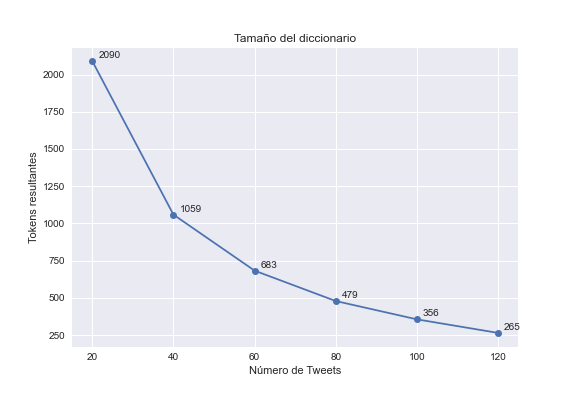
\includegraphics[scale=.4]{../imgs/no_below_len_dict.png}
		\caption{Tamaño del diccionario en función de la cantidad de tweets mínima a la que las palabras deben permanecer. Es decir, $y$ corresponde a las palabras que resultan al filtrar las que aparezcan en menos de $x$ tweets. Este gráfico es importante porque nos permite ver con que tanto vocabulario nos quedamos cuando eliminamos palabras sin mucha importancia o para el modelo.}
	\end{figure}

	

	La siguiente etapa en el preprocesamiento es transformar los tweets en vectores. Para esto, a cada palabra del diccionario $V$ se le asigna un único índice de forma que el conjunto de palabras (o diccionario) se modela como $\set{1,...,|V|}$. Luego, cada tweet, entendido como una colección de palabras en $V$ de la forma $t=\set{v_1,...,v_n}$, se transforma en $\set{(v_1,r_1),...,(v_n,r_n)}$ donde $v_i$ es el índice de la palabra en $V$ y $r_i$ la cantidad de veces que $v_i$ aparece en $t$. A continuación, un ejemplo de esto.
	
	\begin{figure}[H]
		\centering
		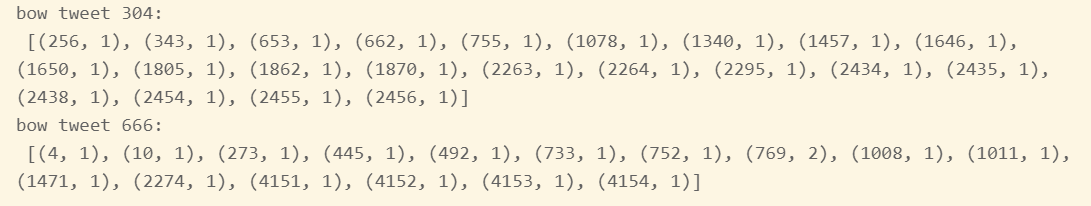
\includegraphics[scale=.5]{../imgs/bow_tweet_informe.png}
		\caption{Estado final de dos tweets escogidos al azar. Esta representación se conoce como \comillas{bow} (\textbf{bag of words}).}
		\label{fig: bow_example}
	\end{figure}
	
	\begin{remark}
		Notar que en los ejemplos que se muestran en la Figura \ref{fig: bow_example}, la segunda componente de las tuplas es mayoritariamente $1$. Esto pasa porque el largo de cada tweet en el corpus es relativamente pequeño en comparación a otros set de datos como por ejemplo una colección de libros o notas periodísticas. Esto sugiere que esta variable no es muy decisiva en este contexto, o bien, que podríamos juntar tweets que estén relativamente cercanos en tiempo, asumiendo que esto implica parentesco temático, para así generar super-tweets de largo mayor. 
	\end{remark}

	\begin{remark}
		Se decide dejar las palabras que hacen referencia a cuentas de Twitter, por ejemplo \texttt{@javier}. La razón de esta decisión es que la aparición de una cuenta en un tópico nos indica que tal persona es relevante para la cuenta sobre la que se está trabajando.
	\end{remark}

\subsection{Aplicando el modelo}
	Como se comentó en la Sección $2$, para aplicar el modelo usamos la implementación de \texttt{gensim}. El código de la Figura \ref{fig: gensim_code_informe} muestra en términos generales lo necesario para correr el algoritmo sobre nuestro corpus.
	
	\begin{figure}[H]
		\centering
		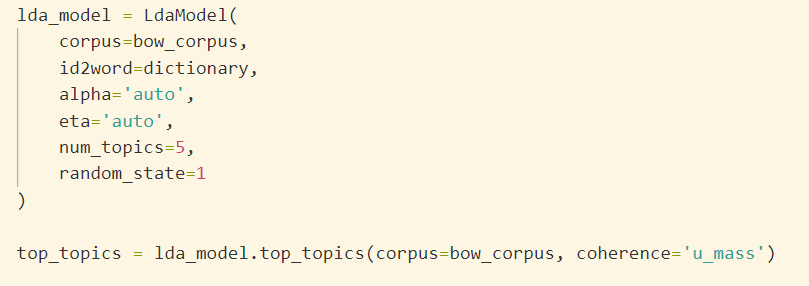
\includegraphics[scale=.4]{../imgs/gensim_code_informe.png}
		\caption{\texttt{corpus} corresponde a lo mostrado en la Figura \ref{fig: bow_example}, \texttt{id2word} es nuestro vocabulario $V$, \texttt{alpha} y \texttt{eta} son los priors discutidos previamente, \texttt{num\_topics} es la cantidad de tópicos que estamos buscando y \texttt{random\_state} es la semilla del algoritmo que en los experimentos siempre fue $1$. El método \texttt{top\_topics} permite obtener coherencia y las distribuciones de cada tópico sobre las palabras.}
		\label{fig: gensim_code_informe}
	\end{figure}
	El parámetro $\alpha$ lo podemos entregar como \texttt{symmetric}, si queremos que sea un vector, calculado internamente con todas sus componentes iguales, \texttt{asymmetric}, si queremos que sea un vector como el anterior salvo que sus componentes son distintas, \texttt{auto} si queremos que el algoritmo calcule un vector tipo \texttt{asymmetric} internamente y un escalar $x$ si queremos que sea tipo \texttt{symmetric} pero que el valor que se repita sea $x$. Por otro lado, $\eta$ puede ser todo lo anterior salvo \texttt{asymmetric}. Acá es importante mencionar que el campo \texttt{coherence} del método \texttt{top\_topics} admite las métricas denominadas: \texttt{u\_mass}, \texttt{c\_v}, \texttt{c\_uci} y \texttt{c\_npmi}. De estas, la única que se pudo implementar sin problemas fue \texttt{u\_mass}, el resto arrojaba un error de \texttt{Python} tipo \texttt{Broken pipe} que no pudo ser solucionado en este proyecto.
	
\subsubsection{Primera iteración}
	 En la Figura \ref{fig: boric0_informe} se muestra el output de pedirle los tópicos a \texttt{gensim}. En esta primera iteración no estamos filtrando palabras de baja frecuencia, los parámetros $(\alpha, \eta)$ se dejan como $(\texttt{auto}, \texttt{auto})$ y pedimos $5$ tópicos. 
	
	\begin{figure}[H]
		\centering
		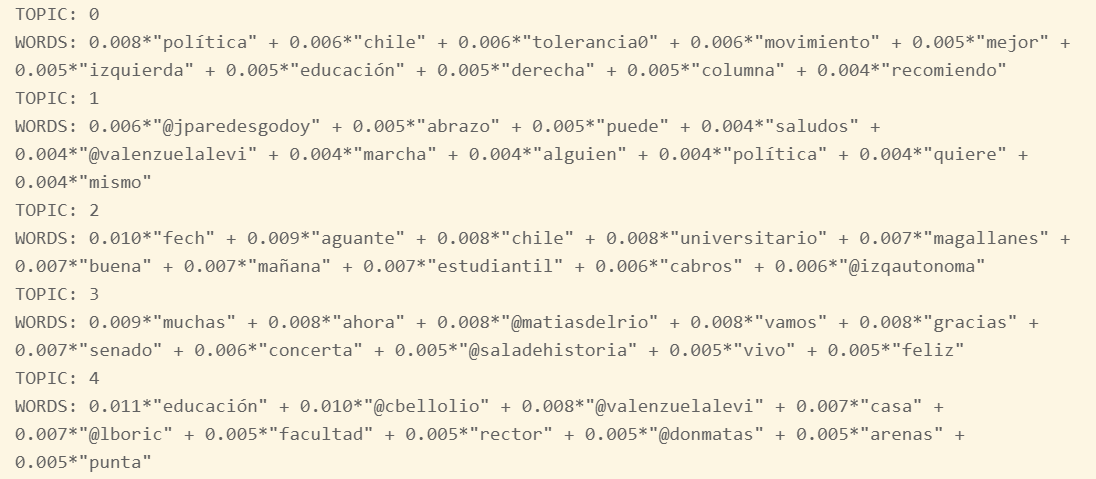
\includegraphics[scale=.32]{../imgs/boric0_informe.png}
		\caption{Los tópicos están ordenados por coherencia y los números que aparecen al lado de cada palabra corresponde a la probabilidad de tal palabra en el tópico. Notar que sólo se muestran las $10$ palabras con mayor probabilidad dentro del tópico, y dado el tamaño de $V$ en este experimento, tales probabilidades son relativamente pequeñas. La coherencia promedio de los tópicos de esta imagen es $-9.1$.}
		\label{fig: boric0_informe}
	\end{figure}

\subsubsection{Segunda iteración}
	Lo que corresponde ahora es optimizar la coherencia promedio de los tópicos con respecto a $(\alpha, \eta)$ y \texttt{num\_topics}. En la primera aproximación a esta tarea calculamos la \texttt{u\_mass} sobre la grilla $\set{5,6,7,8,9,10}\times\set{\texttt{auto}, 0.5}\times\set{\texttt{auto}, 0.5}$ lo cual nos genera $24$ puntos, ver Figura \ref{fig: param_optimization0_informe}.
	
	
	
	\begin{figure}[H]
		\centering
		\subfloat[]{
			\begin{minipage}{0.45\textwidth}
				\label{fig: param_optimization0_informe}
				\centering
				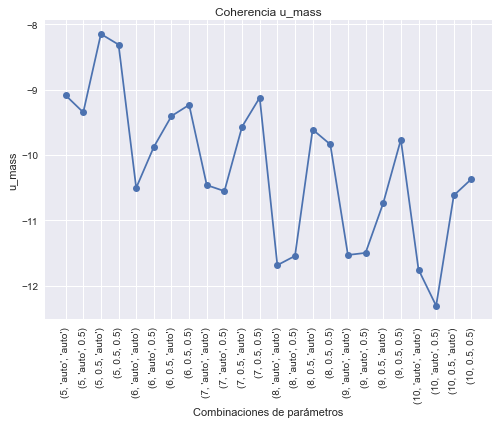
\includegraphics[width=\textwidth]{../imgs/param_optimization0_informe.png}
			\end{minipage}
		}
		\subfloat[]{
			\begin{minipage}{0.45\textwidth}
				\centering
				\label{fig: param_optimization2_informe}
				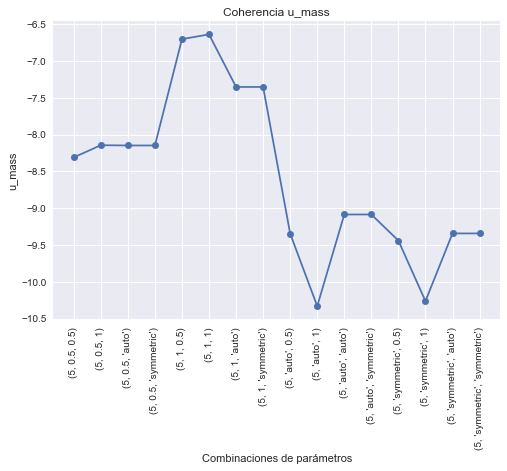
\includegraphics[width=\textwidth]{../imgs/param_optimization2_informe.png}
			\end{minipage}
		}
		\caption{Coherencia por cada combinación de parámetros. Las tuplas del eje $x$ son de la forma $(\texttt{num\_topics}, \alpha, \eta)$. Recordar que esta métrica es tal que mientras más cercana a $0$ mejor. (a) corresponde a la segunda iteración y (b) a la tercera.}
	\end{figure}
 	
 	De la Figura \ref{fig: param_optimization0_informe} deducimos que la cantidad de tópicos escogidos es relevante y que mientras menos tópicos fijamos, más será la coherencia promedio. Es por esto que se decide fijar esta variable a $5$ de aquí en adelante. Otra observación es que para número de tópicos fijos $n\in\set{5,6,7,8,9,10}$, las mejores combinaciones son $(n, 0.5, \texttt{auto})$ y $(n, 0.5, 0.5)$. El mejor modelo en esta iteración es $(\texttt{num\_topics}=5,\alpha= 0.5, \eta=\texttt{auto})$ con coherencia de $-8.15$.
 	
 \subsubsection{Tercera iteración}
	Dado que fijamos el número de tópicos en $5$, en esta iteración nos preocupamos solamente de optimizar con respecto a $(\alpha, \eta)$. Primero vamos a comparar entre fijar los parámetros como sólo números y fijar al menos uno de estos como \texttt{auto}, \texttt{symmetric} o \texttt{asymmetric}, para esto experimentamos con $(\alpha, \eta)\in\set{0.5, 1,\texttt{auto}, \texttt{symmetric}}^2$. Como los máximos en la Figura \ref{fig: param_optimization2_informe} son alcanzados cuando tanto $\alpha$ como $\eta$ son números, se decide trabajar ambas variables de esta forma. Además, pareciera que mientras más grande sean estos números, mejor es la coherencia, en este caso el máximo se alcanza cuando ambos valores son iguales a $1$ que es lo más alto que se usó.
	
	\begin{figure}[H]
		\centering
		\subfloat[]{
			\begin{minipage}{0.45\textwidth}
				\label{fig: param_optimization3_informe}
				\centering
				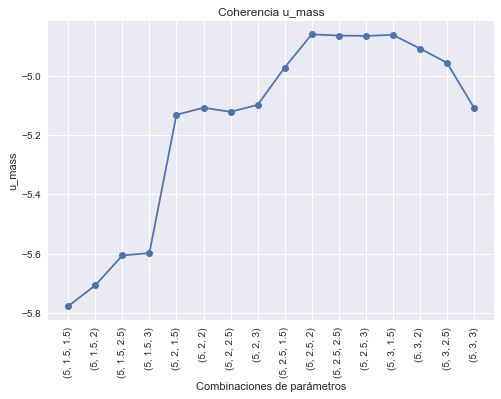
\includegraphics[width=\textwidth]{../imgs/param_optimization3_informe.png}
			\end{minipage}
		}
		\subfloat[]{
			\begin{minipage}{0.45\textwidth}
				\centering
				\label{fig: boric3_informe}
				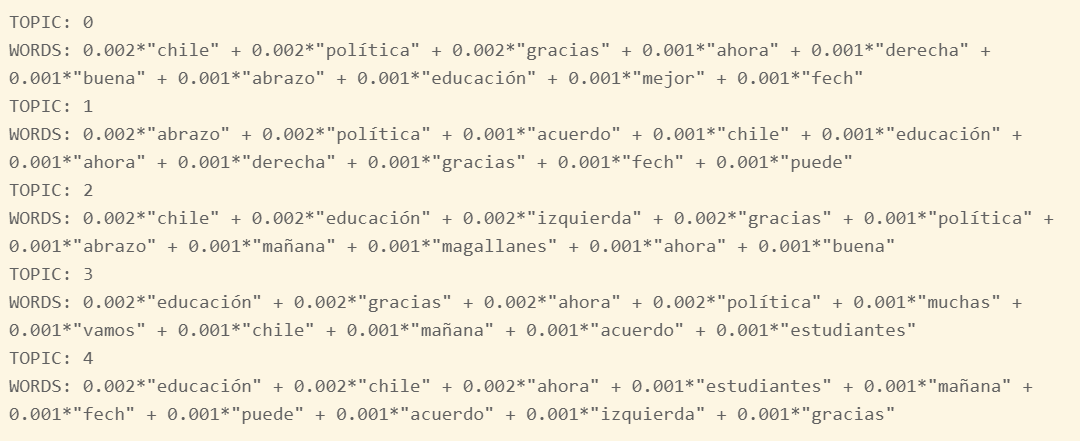
\includegraphics[width=\textwidth, height=4cm]{../imgs/boric3_informe.png}
			\end{minipage}
		}
		\caption{Coherencia (a) y tópicos asociados a los mejores parámetros encontrados (b).}
	\end{figure}
	 
	
	En la Figure \ref{fig: param_optimization3_informe} se tomó $(\alpha, \eta)\in\set{1.5, 2, 2.5, 3}^2$ y confirma que si usamos valores más altos para $\alpha$ y $\eta$ la coherencia aumenta, pero hasta cierto punto porque el crecimiento se detiene cuando ambos llegan a $3$. Los mejores parámetros de esta iteración son $(\texttt{num\_topics}=5,\alpha=2.5, \eta=2)$ con una coherencia promedio de $-4.86$. La mala noticia acá es que los tópicos, representados por las $10$ palabras más probables, son prácticamente los mismos (ver Figura \ref{fig: boric3_informe}) y comparten varias palabras. Esto se puede explicar teniendo en cuenta que los tweets son de una persona en particular, que además viene de un ámbito mayoritariamente político, y por consiguiente sus tweets tienen esta misma connotación.
	
	
\subsubsection{Cuarta iteración (cambio de data set)}
	Dado lo discutido en la parte anterior, se decide aplicar los métodos anteriores a otro data set. Este data set consiste en tweets creados en Santiago durante un periodo de ocho días, en específico, del $3$ de enero de $2021$ hasta el $10$ del mismo mes y año. Por lo tanto, se espera haya una cantidad más variada de temas y palabras con respecto a los resultados anteriores. El procedimiento es el mismo de la iteración pasada, se preprocesan los tweets y se optimiza la coherencia promedio con respecto a $(\alpha, \eta)$ fijando $\texttt{num\_topics}=5$ por simpleza. La única diferencia es que en este caso se filtrarán (quitándo) las palabras que estén presentes en menos de $100$ tweets luego del preprocesamiento, esto nos llevó a reducir el vocabulario de $80920$ a $656$ palabras.  
	
	\begin{figure}[H]
		\centering
		\subfloat[]{
			\begin{minipage}{0.45\textwidth}
				\label{fig: mix_param_optimization0_informe}
				\centering
				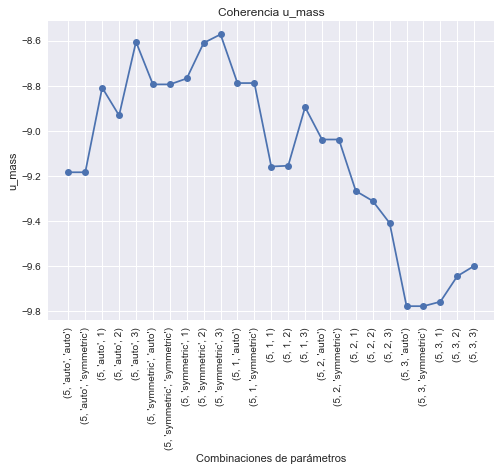
\includegraphics[width=\textwidth]{../imgs/mix_param_optimization0_informe.png}
			\end{minipage}
		}
		\subfloat[]{
			\begin{minipage}{0.45\textwidth}
				\centering
				\label{fig: mix0_informe}
				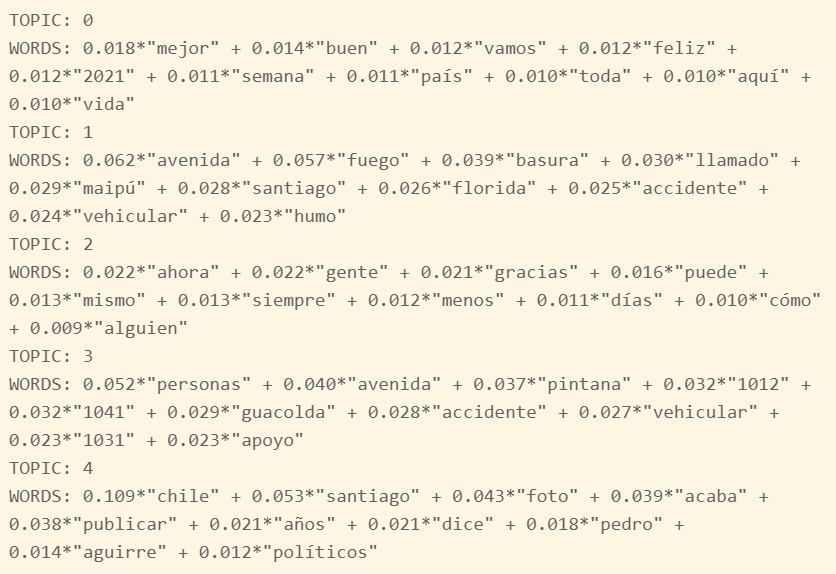
\includegraphics[width=\textwidth]{../imgs/mix0_informe.png}
			\end{minipage}
		}
		\caption{Coherencia (a) y tópicos asociados a los mejores parámetros encontrados (b).}
	\end{figure}

	En la Figura \ref{fig: mix_param_optimization0_informe} se usó $(\alpha,\eta)\in\set{\texttt{auto}, \texttt{symmetric}, 1, 2, 3}^2$ y los mejores parámetros resultaron $(\alpha=\texttt{symmetric},\eta=3)$ con una coherencia igual a $-8.6$. En la Figura \ref{fig: mix0_informe} podemos ver una mayor diversidad de palabras, incluso el tópico $0$, que tiene la coherencia más alta igual a $-4.6$, tiene un carácter positivo en cuanto a sus primeras $4$ palabras con mayor probabilidad. El tópico $1$, al estar presenta el par \textbf{accidente vehicular}, podemos concluir que nos esta hablando justamente de situaciones de accidentes. El resto de los tópicos no tienen un carácter bien definido salvo por el $4$, este nos está hablando, quizá con un poco menos de seguridad, de publicaciones de fotos. También notamos que las probabilidades son relativamente mayores en comparación a lo obtenido en la sección de \texttt{@gabrielboric}, esto se explica por la reducción de vocabulario en esta iteración.
	
	
\section{Conclusión}
	
	Claramente, la decisión de analizar sólo una cuenta para así disminuir la complejidad de la cantidad de tópicos, no fue la más acertada. Si bien la optimización de los parámetros conllevó un aumento significativo en la coherencia, los tópicos de la cuenta \texttt{@gabrielboric} tendieron a ser muy parecidos pudiendo ser caracterizados como \comillas{Política y Educación}. Un análisis más profundo lleva a pensar que se cumple la hipótesis de que los temas de esta cuenta estarían ligados a la política, pero, es tan así que este pareciera ser el único tema que se discute en el data set.\\
	
	Cuando se pasa a analizar todos los tweets creados en Santiago durante un periodo de tiempo, somos capaces de encontrar más palabras y los tópicos rara vez se sobreponen entre si, pero cuesta darle una interpretación a los tópicos en base a sus palabras de mayor probabilidad. Esto lo podemos explicar por la naturaleza \textbf{unsupervised learning} del modelo, puesto que no tenemos nuestro tweets o palabras clasificadas en ciertos tópicos predeterminados y el algoritmo trata por si sólo de encontrar y generar estos tópicos, que como vemos no siempre son interpretables. Además, se concluye que la métrica de coherencia por sí sola no es suficiente, se hace necesario un humano/a para poder encasillar e interpretar los tópicos que nos entrega LDA.\\
	
	En resumen, se logra optimizar de buena forma la métrica \texttt{u\_mass} pero no así la del ojo humano. Para expandir este proyecto se podría trabajar con tweets de diferentes cuentas que se sepa de ante mano que tocan temas distintos entre si y tratar de capturarlos, otra cosa que se podría hacer es un preprocesamiento más fino o tratar de unir tweets para no tener textos tan cortos.
	   
\begin{thebibliography}{99}
	
\end{thebibliography}
\end{document}
